% !TEX root = ../../../main.tex

\toggletrue{image}
\togglefalse{imagehover}
\chapterimage{decoder_calvin_hobbes}
\chapterimagetitle{ENCRYPTION RING}
\chapterimageurl{https://calvinandhobbes.fandom.com}

\chapter{Monoalphabetische Kryptosysteme}
\label{chapter-monoalphabetische-kryptosysteme}

Wir starten mit einem Kryptosystem, welches der Überlieferung nach von Gaius Julius Caesar für seine militärische Korrespondenz benutzt wurde. Wir führen eine erste Kryptoanalyse durch und verbessern dann das Kryptosystem schrittweise. Abschliessend halten wir fest, warum \textbf{alle} symmetrischen und monoalphabetischen Kryptosysteme nicht sicher sind. Die Lernziele lauten:

\newcommand{\monoalphabetischeKryptosystemeLernziele}{
\protect\begin{todolist}
\item Sie erklären, was wir unter einem monoalphabetischen Kryptosystem verstehen.
\item Sie erklären, was wir unter der Schlüsselmenge verstehen.
\item Sie erklären jedes vorgestellte monoalphabetische Kryptosystem und wenden es an.
\item Sie führen eine Kryptoanalyse für alle monoalphabetischen Kryptosysteme durch.
\item Sie entwerfen ein monoalphabetisches Kryptosystem.
\end{todolist}
}

\lernziel{\autoref{chapter-monoalphabetische-kryptosysteme}, \nameref{chapter-monoalphabetische-kryptosysteme}}{\protect\monoalphabetischeKryptosystemeLernziele}

\monoalphabetischeKryptosystemeLernziele

\section{Das Kryptosystem \texttt{CAESAR}}

Das wahrscheinlich bekannteste Beispiel für ein monoalphabetisches Kryptosystem\footnote{Auch wenn nicht jedes Mal explizit notiert, gehen wir immer von einem symmetrischen Kryptosystem aus.} ist das Kryptosystem  \texttt{CAESAR}. Es ist nach dem römischen Feldherrn Gaius Julius Caesar benannt und vorwiegend durch die Darstellung als Scheibe (siehe \autoref{figure-caesar-beispiel}) bekannt. 


\begin{figure}[htb]
\centering
\Caesar{26}{-1}{off}{off}
\caption{Zwei drehbare Scheiben, welche in der Mitte miteinander verbunden sind.}
\label{figure-caesar-beispiel}
\end{figure}

Die Alphabete für das Kryptosystem \texttt{CAESAR} lauten:

\begin{itemize}
\item Klartextalphabet: A, B, C, D, E, F, G, H, I, K, L, M, \dots , S, T, U, V, W, X, Y, Z
\item Kryptotextalphabet: A, B, C, D, E, F, G, H, I, K, L, M, \dots , S, T, U, V, W, X, Y, Z
\end{itemize}

\subsection{Verschlüsselung und Entschlüsselung}

Das Prinzip beruht darauf, in dem \textbf{Buchstabe für Buchstabe} durch einen \textbf{anderen Buchstaben ersetzt} wird. Die Drehung der inneren Scheibe bestimmt dabei, welcher Buchstabe wie ersetzt wird.

\begin{definition}[Schlüssel für \texttt{CAESAR}]
Die \textbf{Anzahl der Verschiebungen} der \textbf{inneren} Scheibe nach \textbf{links} ist der Schlüssel des Kryptosystems \texttt{CAESAR}. Den Schlüssel geben wir somit einfach durch eine Zahl an.
\end{definition}

\begin{example}
In \autoref{figure-caesar-beispiel-encrypt} ist der Schlüssel \num{5}, in \autoref{figure-caesar-beispiel-decrypt} lautet der Schlüssel \num{10}.
\end{example}

\begin{figure}[htb]
\begin{minipage}{0.45\textwidth}
\centering
\Caesar{-5}{5}{O}{J}
\caption{Der Schlüssel lautet \num{5}.}
\label{figure-caesar-beispiel-encrypt}
\end{minipage}
\hfill
\begin{minipage}{0.45\textwidth}
\centering
\Caesar{-10}{10}{K}{A}
\caption{Der Schlüssel lautet \num{10}.}
\label{figure-caesar-beispiel-decrypt}
\end{minipage}
\end{figure}

Wir \textbf{verschlüsseln} einen Klartextbuchstaben, in dem wir auf der \textbf{inneren} Scheibe den Klartextbuchstaben suchen und auf der \textbf{äusseren} den dazugehörigen Kryptotextbuchstaben ablesen.

\begin{example}
Wenn wir mit \autoref{figure-caesar-beispiel-encrypt} den Klartextbuchstaben J verschlüsseln, dann erhalten wir das O. Das Wort JULIUS verschlüsseln wir somit zu OZQNZX.
\end{example}

Wir \textbf{entschlüsseln} einen Kryptotextbuchstaben, in dem wir auf der \textbf{äusseren} Scheibe den Kryptotextbuchstaben suchen und auf der \textbf{inneren} den dazugehörigen Klartextbuchstaben ablesen.

\begin{example}
Wenn wir mit \autoref{figure-caesar-beispiel-decrypt} den Kryptotextbuchstaben K entschlüsseln, dann erhalten wir das A. Das Wort KDVKC entschlüsseln wir somit zu ATLAS.
\end{example}

\begin{definition}[Schlüsselmenge für \texttt{CAESAR}]
Das Kryptosystem \texttt{CAESAR} besitzt die Schlüsselmenge $\mathscr{S}_{\texttt{CAESAR}} = \{1, 2, 3, \dots , 24, 25, 26\}$, da wir für die innere Scheibe insgesamt $26$ verschiedene Positionen einstellen können ($|\mathscr{S}_{\texttt{CAESAR}}| = 26$).
\end{definition}

\subsection{Kryptoanalyse}

Ist das Kryptosystem \texttt{CAESAR} sicher? Gemäss dem Prinzip von Kerkhoff, ist die Funktionsweise des Kryptosystems öffentlich bekannt. Wir können also gezielt, eine Schwachstelle des Kryptosystems auszunutzen. Die einfachste Attacke besteht darin, alle möglichen Schlüssel auszuprobieren.

\begin{definition}[Brute-Force-Methode]
	Probieren wir systematisch alle Möglichkeiten für den Schlüssel durch, dann sprechen wir von der Brute-Force-Methode (\say{Methode der rohen Gewalt}). Mit dieser Methode knacken wir (zumindest theoretisch) jedes Kryptosystem. Wir brauchen im schlimmsten Fall $n$ Versuche, wobei wir mit $n$ die Anzahl der Schlüssel meinen (d.h. $|\mathscr{S}|=n$).
\end{definition}

Da $|\mathscr{S}_{\texttt{CAESAR}}| = 26$ gilt, können wir mithilfe der \textbf{Brute-Force-Methode} das Kryptosystem \texttt{CAESAR} für \textbf{jeden} Kryptotext problemlos knacken. Wir probieren einfach so lange einen Schlüssel nach dem anderen aus, bis eine Entschlüsselung Sinn ergibt.

\newpage

\begin{example}[Brute-Force-Methode für \texttt{CAESAR}]
Es ist der Kryptotext NORAQRFFRAHZNPUGORVZVE gegeben\footnote{Angriff mit bekanntem Kryptotext}. Wir probieren alle Schlüssel aus und erhalten folgende Klartexte:

\begin{multicols}{2}
\begin{enumerate}
\item MNQZPQEEQZGYMOTFNQUYUD
\item LMPYOPDDPYFXLNSEMPTXTC
\item KLOXNOCCOXEWKMRDLOSWSB
\item JKNWMNBBNWDVJLQCKNRVRA
\item IJMVLMAAMVCUIKPBJMQUQZ
\item HILUKLZZLUBTHJOAILPTPY
\item GHKTJKYYKTASGINZHKOSOX
\item FGJSIJXXJSZRFHMYGJNRNW
\item EFIRHIWWIRYQEGLXFIMQMV
\item DEHQGHVVHQXPDFKWEHLPLU
\item CDGPFGUUGPWOCEJVDGKOKT
\item BCFOEFTTFOVNBDIUCFJNJS
\item \textbf{ABENDESSENUMACHTBEIMIR}
\item ZADMCDRRDMTLZBGSADHLHQ
\item YZCLBCQQCLSKYAFRZCGKGP
\item XYBKABPPBKRJXZEQYBFJFO
\item WXAJZAOOAJQIWYDPXAEIEN
\item VWZIYZNNZIPHVXCOWZDHDM
\item UVYHXYMMYHOGUWBNVYCGCL
\item TUXGWXLLXGNFTVAMUXBFBK
\item STWFVWKKWFMESUZLTWAEAJ
\item RSVEUVJJVELDRTYKSVZDZI
\item QRUDTUIIUDKCQSXJRUYCYH
\item PQTCSTHHTCJBPRWIQTXBXG
\item OPSBRSGGSBIAOQVHPSWAWF
\item NORAQRFFRAHZNPUGORVZVE
\end{enumerate}
\end{multicols}

Wir erkennen, dass mit dem Schlüssel \num{13} ein sinnvoller Text entsteht (Abendessen um acht bei mir). Wir könnten das Verfahren nun stoppen. Das Beispiel zeigt jedoch alle möglichen Klartexte. Mit einem Computerprogramm ist es hier einfacher, einfach alle Möglichkeiten anzeigen zu lassen und selbst den korrekten Klartext zu ermitteln.
\end{example}

\begin{important}
Das Kryptosystem \texttt{CAESAR} ist \textbf{nicht} sicher. Eve kann durch das Ausprobieren aller Schlüssel den Klartext ermitteln. Dabei braucht sie keinerlei Kenntnisse über den konkreten Schlüssel.
\end{important}

\subsection{Ausblick}

Durch die geringe Anzahl von Schlüsseln können wir das Kryptosystem \texttt{CAESAR} mithilfe der Brute-Force-Methode knacken. Wir können diese Attacke dadurch unmöglich machen, in dem wir die Anzahl der Schlüssel so gross machen, dass kein Computer in vernünftiger Zeit alle Schlüssel ausprobieren kann. In \autoref{sec-caesar-abstract} und \autoref{sec-caesar-abstract} werden wir dieses Ziel schrittweise erreichen.

\newpage

\subsection{Aufgaben}

Für die folgenden Aufgaben ist immer das Kryptosystem \texttt{CAESAR} zu verwenden. Sie können die Caesar-Scheiben aus \autoref{figure-caesar-scheiben-aufgaben} verwenden.

\begin{figure}[htb]
\centering
\begin{minipage}{0.3\textwidth}
\centering
\resizebox{3.5cm}{!}{
\Caesar{-10}{10}{off}{off}
}
\end{minipage}
\begin{minipage}{0.3\textwidth}
\centering
\resizebox{3.5cm}{!}{
\Caesar{-17}{17}{off}{off}
}
\end{minipage}
\begin{minipage}{0.3\textwidth}
\centering
\resizebox{3.5cm}{!}{
\Caesar{-9}{9}{off}{off}
}
\end{minipage}
\caption{Caesar-Scheiben für die Aufgaben.}
\label{figure-caesar-scheiben-aufgaben}
\end{figure}

\begin{enumerate}
\item Verschlüsseln Sie den Klartext ABENTEUER. Verwenden Sie den Schlüssel \num{10}.

\fillwithlines{0.25in}

\item Bestimmen Sie die Verschlüsselung von STANLEY mit dem Schlüssel \num{17}.

\fillwithlines{0.25in}

\item Entschlüsseln Sie den Kryptotext NGCAJLCRXW DWM RWLNYCRXW. Es wurde der Schlüssel \num{9} benutzt.

% EXTRACTION UND INCEPTION

\fillwithlines{0.25in}

\item Um das Jahr 1980 herum wurde in den Newsgroups des Internets die \texttt{ROT13}-Chiffrierung verwendet, um zum Beispiel Pointen von Witzen zu verschleiern (\say{Spoiler-Schutz}). \texttt{ROT13} ist eine Geheimschrift. Es entspricht dem Kryptosystem \texttt{CAESAR} unter der Verwendung des \textbf{fixen} Schlüssels \num{13}. Was ist das Besondere am Schlüssel \num{13} beim Kryptosystem \texttt{CAESAR}? Versuchen Sie es herauszufinden, indem Sie TRAUM verschlüsseln und den daraus resultierenden Kryptotext erneut verschlüsseln.

\fillwithlines{2in}

\item Der Kryptotext EXRRPSXAAN RXGRJH ist mit dem Kryptosystem \texttt{CAESAR} verschlüsselt worden. Knacken Sie den Kryptotext mit der Brute-Force-Methode.

%PICCADILLY CIRCUS

\fillwithlines{0.75in}

\item Sie haben \num{13} Personen und möchten einen Kryptotext knacken, welcher mit \texttt{CAESAR} verschlüsselt wurde. Wie könnten Sie effizient vorgehen?

\fillwithlines{\stretch{1}}

\end{enumerate}

\newpage

\section{Das Kryptosystem \texttt{CAESAR-ABSTRAKT}}
\label{sec-caesar-abstract}

Wir können durch Abstraktion das Kryptosystem \texttt{CAESAR} auch \textbf{ohne} die Scheibe einsetzen.

\begin{definition}[Abstraktion]
In der zur Verfügung stehenden Information stecken oft sowohl relevante als auch irrelevante Anteile. Durch Abstraktion \textbf{reduzieren} wir die \textbf{Information} auf das für die aktuelle Situation \textbf{wesentliche}.
\end{definition}

Das Wesentliche bei der Caesar-Scheibe ist die Verschiebung der Buchstaben und das anschliessende Ersetzen der Buchstaben. Dies erreichen wir auch dadurch, in dem wir die Caesar-Scheibe tabellarisch darstellen. \autoref{table-caesar-bsp-5} zeigt dies für die Caesar-Scheibe aus \autoref{figure-caesar-bsp-5}.

\begin{table}[htb]
\centering
\begin{tblr}{
    colspec = {|c|c|c|c|c|c|c|c|c|c|c|c|c|c|c|c|c|c|c|c|c|c|c|c|c|c|c|}
}
\hline
Klartextbuchstabe & A & B & C & D & E & F & G & H & I & J & K & L & M \\ \hline
Kryptotextbuchstabe & F & G & H & I & J & K & L & M & N & O & P & Q & R  \\ \hline[2pt]
Klartextbuchstabe & N & O & P & Q & R & S & T & U & V & W & X & Y & Z \\ \hline
Kryptotextbuchstabe & S & T & U & V & W & X & Y & Z & A & B & C & D & E  \\ \hline
\end{tblr}
\caption{Der Schlüssel ist $5$.}
\label{table-caesar-bsp-5}
\end{table}

\vspace{-1cm}

\begin{figure}[htb]
\centering
\begin{minipage}{0.45\textwidth}
\centering
\resizebox{3cm}{!}{
\Caesar{-5}{5}{off}{off}
}
\caption{Der Schlüssel lautet \num{5}.}
\label{figure-caesar-bsp-5}
\end{minipage}
\hfill
\begin{minipage}{0.45\textwidth}
\centering
\resizebox{3cm}{!}{
\Caesar{-10}{10}{off}{off}
}
\caption{Der Schlüssel lautet \num{10}.}
\label{figure-caesar-bsp-10}
\end{minipage}
\end{figure}

Der \textbf{Schlüssel} bei \texttt{CAESAR-ABSTRAKT} ist immer noch eine Zahl. Die Zahl gibt an, um wie viele \textbf{Positionen die Buchstaben} in der \textbf{unteren Zeile} der Tabelle nach \textbf{links} verschoben werden. 

\begin{important}
Wir haben lediglich die Darstellung des Kryptosystems verändert. Die Eigenschaften des Kryptosystems \texttt{CAESAR-ABSTRAKT} sind identisch zum Kryptosystem \texttt{CAESAR}.
\end{important}

Warum haben wir diesen Aufwand betrieben? Durch diese Darstellung können wir die Anzahl der Schlüssel auf einfache Weise drastisch erhöhen. In \autoref{sec-caesar-plus} wird gezeigt wie.

\subsection{Aufgaben}

\begin{enumerate}
\item Stellen Sie \texttt{CAESAR} aus \autoref{figure-caesar-bsp-10} als \texttt{CAESAR-ABSTRAKT} dar.

\begin{table}[htb]
\centering
\begin{tblr}{
    colspec = {|c|c|c|c|c|c|c|c|c|c|c|c|c|c|c|c|c|c|c|c|c|c|c|c|c|c|c|}
}
\hline
Klartextbuchstabe & A & B & C & D & E & F & G & H & I & J & K & L & M \\ \hline
Kryptotextbuchstabe &  &  &  &  &  &  &  &  &  &  &  &  &   \\ \hline[2pt]
Klartextbuchstabe & N & O & P & Q & R & S & T & U & V & W & X & Y & Z \\ \hline
Kryptotextbuchstabe & &  & & & & & & & & & & &  \\ \hline
\end{tblr}
\end{table}

\item Wie lautet der Schlüssel für \texttt{CAESAR-ABSTRAKT} mit nachfolgender Tabelle.

\fillwithlines{0.25in}

\begin{table}[H]
\centering
\begin{tblr}{
    colspec = {|c|c|c|c|c|c|c|c|c|c|c|c|c|c|c|c|c|c|c|c|c|c|c|c|c|c|c|}
}
\hline
Klartextbuchstabe & A & B & C & D & E & F & G & H & I & J & K & L & M \\ \hline
Kryptotextbuchstabe & R & S & T & U & V & W & X & Y & Z & A & B & C & D   \\ \hline[2pt]
Klartextbuchstabe & N & O & P & Q & R & S & T & U & V & W & X & Y & Z \\ \hline
Kryptotextbuchstabe & E & F & G & H & I & J & K & L & M & N & O & P & Q \\ \hline
\end{tblr}
\end{table}

\end{enumerate}

\section{Das Kryptosystem \texttt{CAESAR-PLUS}}
\label{sec-caesar-plus}

Beim Kryptosystem \texttt{CAESAR-ABSTRAKT} gibt es \textbf{nur} $26$ verschiedene Schlüssel (Tabellen). Wir wollen nun ein Kryptosystem mit wesentlich mehr Schlüsseln erstellen. Dazu können wir die einfache \textbf{Verschiebung des Alphabets} aufheben und eine \textbf{beliebige Zuordnung der Buchstaben} erlauben. Dadurch erhalten wir das Kryptosystem \texttt{CAESAR-PLUS}.

\begin{example}
\autoref{table-caesar-plus-bsp-1} zeigt eine Möglichkeit für eine Zuordnung der Kryptotextbuchstaben.
\end{example}

\vspace{-0.3cm}

\begin{table}[htb]
\centering
\begin{tblr}{
    colspec = {|c|c|c|c|c|c|c|c|c|c|c|c|c|c|c|c|c|c|c|c|c|c|c|c|c|c|c|}
}
\hline
Klartextbuchstabe 	& A & B & C & D & E & F & G & H & I & J & K & L & M \\ \hline
Kryptotextbuchstabe & P & Z & Q & N & H & J & V & T & A & E & C & O & L  \\ \hline[2pt]
Klartextbuchstabe 	& N & O & P & Q & R & S & T & U & V & W & X & Y & Z \\ \hline
Kryptotextbuchstabe & G & X & B & R & U & I & F & M & W & D & Y & S & K  \\ \hline
\end{tblr}
\caption{Wir ordnen die \num{26} Kryptotextbuchstaben in einer beliebigen Reihenfolge an.}
\label{table-caesar-plus-bsp-1}
\end{table}

\vspace{-0.8cm}

\subsection{Verschlüsselung und Entschlüsselung}

Die \textbf{Verschlüsselung} eines Klartextes erfolgt Buchstabe für Buchstabe. Wir suchen den Klartextbuchstaben in der Tabelle und ersetzen diesen durch den \textbf{darunter} liegenden Kryptotextbuchstaben.

\begin{example}
Der Klartext BUCH wird mit \autoref{table-caesar-plus-bsp-1} zu ZMQT verschlüsselt.
\end{example}

Wir \textbf{entschlüsseln} einen Kryptotext, in dem wir Kryptotextbuchstabe für Kryptotextbuchstabe in der Tabelle suchen und jeweils durch den \textbf{darüber} liegenden Klartextbuchstaben ersetzen.

\begin{example}
Der Kryptotext IFAJF wird mit \autoref{table-caesar-plus-bsp-1} zu STIFT entschlüsselt.
\end{example}

\begin{definition}[Schlüssel für \texttt{CAESAR-PLUS}]
Den Schlüssel, den Alice und Bob vereinbaren müssen, ist die Tabelle mit den Zuordnungen der Klartext- und Kryptotextbuchstaben.
\end{definition}

\vspace{-0.7cm}

\subsection{Schlüsselmenge}

Wir haben das Kryptosystem \texttt{CAESAR-PLUS} mit dem Ziel entwickelt, die Anzahl der Schlüssel deutlich zu erhöhen. Deshalb bestimmen wir nun, wie gross die Schlüsselmenge ist.

\begin{definition}[Schlüsselmenge für \texttt{CAESAR-PLUS}]
Die Schlüsselmenge $\mathscr{S}_{\texttt{CAESAR-PLUS}}$ beinhaltet alle verschiedenen Zuordnungen (Tabellen) der \num{26} Klartext- und Kryptotextbuchstaben. Die Schlüsselmenge besitzt die Grösse $|\mathscr{S}_{\texttt{CAESAR-PLUS}}|=26! = 26 \cdot 25 \cdot 24 \cdots 3 \cdot 2 \cdot 1 = \num{403291461126605635584000000} \approx 4 \cdot 10^{26} \approx 403$ Quadrillionen.
\end{definition}

\vspace{-0.2cm}

Wir erklären nun, wie wir auf $26!$\footnote{Das Ausrufezeichen wird in der Mathematik als Fakultät bezeichnet. $26!$ wird als \say{26 Fakultät} ausgesprochen.} als Grösse für die Schlüsselmenge kommen.

\begin{definition}[Permutation von Buchstaben]
	Eine Permutation ist eine beliebige \say{Umordnung} der Buchstaben. Es geht dabei um die Anordnung der Buchstaben in einer bestimmten Reihenfolge. Bei $n$ Buchstaben gibt es $n! = n \cdot (n-1) \cdot (n-2) \cdots 2 \cdot 1$ verschiedene Permutationen, das heisst $n!$ verschiedene Möglichkeiten, die $n$ Buchstaben anzuordnen.
\end{definition}

\vspace{-0.2cm}

Damit wir uns besser vorstellen können, was wir unter einer Permutation verstehen, geben wir ein vollständiges Beispiel mit vier Buchstaben.

\begin{example}
In \autoref{table-kombinationen-vier-buchstaben} sind alle Möglichkeiten aufgelistet, wie wir die vier Buchstaben A, B, C und D anordnen können. Jede Zelle entspricht einer Permutation der vier Buchstaben.
\end{example}

\begin{table}[H]
\centering
\begin{tblr}{
    colspec = {|c|c|c|c|c|c|c|c|}
}
\hline
ABCD & ABDC & ACDB & BCDA & BACD & BADC & CADB & CBDA \\ \hline
ACBD & ADBC & ADCB & BDCA & BCAD & BDAC & CDAB & CDBA  \\ \hline
CABD & DABC & DACB & DBCA & CBAD & DBAC & DCAB & DCBA  \\ \hline
\end{tblr}
\caption{Es gibt $4! = 4 \cdot 3 \cdot 2 \cdot 1 = 24$ Permutationen für vier Buchstaben.}
\label{table-kombinationen-vier-buchstaben}
\end{table}

Da wir bei \texttt{CAESAR-PLUS} die \num{26} Kryptotextbuchstaben in einer beliebigen Reihenfolge anordnen dürfen, entspricht die Grösse der Schlüsselmenge gerade die Anzahl der Permutationen für \num{26} verschiedene Buchstaben, das heisst $26!$. 

\subsection{Kryptoanalyse}

Ist das Kryptosystem \texttt{CAESAR-PLUS} deshalb sicher? Wir versuchen wieder den Klartext für einen gegebenen Kryptotext zu ermitteln (Angriff mit bekanntem Kryptotext).

\begin{important}
Die Brute-Force-Methode für das Knacken eines Kryptotextes ist ausgeschlossen. Nehmen wir einmal an, dass ein Computer in einer Nanosekunde ($\qty{1}{\ns} = \qty{0,000000001}{\s}$) exakt einen Schlüssel testen kann, dann benötigt der Computer etwa \num{13} Milliarden Jahre für alle Schlüssel. Das systematische Ausprobieren aller Schlüssel ist somit keine akzeptable Methode für das Knacken von \texttt{CAESAR-PLUS}.
\end{important}

Dazu hilft zunächst folgende Beobachtung: Bei \texttt{CAESAR-PLUS} wird für einen beliebigen, aber \textbf{fixen} Schlüssel jeder \textbf{Klartextbuchstabe} \textbf{immer} mit \textbf{demselben} \textbf{Kryptotextbuchstaben} verschlüsselt.

\begin{example}
Wir verschlüsseln den Klartext DAMPFSCHIFFFAHRT mit dem Schlüssel aus \autoref{table-caesar-plus-bsp-1}. Wir erhalten den Kryptotext NPLBJIQTAJJJPTUF. Jedes F im Klartext wurde zu einem J verschlüsselt.
\end{example}

Diese Eigenschaft von \texttt{CAESAR-PLUS} können wir für einen Angriff ausnutzen.

\begin{definition}[Monoalphabetische Kryptosysteme]
Ein Kryptosystem heisst monoalphabetisch, wenn \textbf{jeder Klartextbuchstabe} (mit beliebigem, aber fixen Schlüssel) \textbf{unabhängig} von seiner Position im Klartext \textbf{immer} durch \textbf{denselben Kryptotextbuchstaben} verschlüsselt wird.
\end{definition}

Bei \texttt{CAESAR}, \texttt{CAESAR-ABSTRAKT} und \texttt{CAESAR-PLUS} sind monoalphabetische Kryptosysteme. Die Kryptoanalyse funktioniert bei monoalphabetischen Kryptosystemen immer gleich. Wir nehmen einmal an, dass es sich beim \textbf{Klartext} um einen \textbf{deutschen Text} handelt. Dann können wir ausnutzen, dass bei deutschen Texten die \textbf{einzelnen Buchstaben unterschiedlich häufig} vorkommen. Der Buchstabe E tritt wesentlich häufiger auf als etwa der Buchstabe Q. In \autoref{table-relative-haeufigkeiten} sind die relativen Häufigkeiten der einzelnen Buchstaben für längere, typische deutsche Texte aufgelistet. 

\begin{table}[htb]
\centering
\resizebox{\textwidth}{!}{
\begin{tblr}{
colspec = {|c|c|c|c|c|c|c|c|}
}
\hline
Buchstabe &  rel. Häufigkeit (\%) &  Buchstabe &  rel. Häufigkeit (\%) &  Buchstabe &  rel. Häufigkeit (\%) &  Buchstabe &  rel. Häufigkeit (\%) \\ \hline
E         & $17,74$                & H         & $5,22$                 & O         & $2,39$                 & V         & $0,64$                 \\ \hline
N         & $10,01$                & D         & $5,12$                 & B         & $1,85$                 & J         & $0,23$                 \\ \hline
I         & $7,60$                 & U         & $4,27$                 & W         & $1,73$                 & Y         & $0,04$                 \\ \hline
R         & $6,98$                 & L         & $3,49$                 & F         & $1,56$                 & X         & $0,02$                 \\ \hline
S         & $6,88$                 & C         & $3,26$                 & K         & $1,40$                 & Q         & $0,01$                 \\ \hline
A         & $6,43$                 & M         & $2,75$                 & Z         & $1,10$                 &           &                      \\ \hline
T         & $5,94$                 & G         & $2,69$                 & P         & $0,64$                 &           &                      \\ \hline
\end{tblr}
}
\caption{Relative Häufigkeiten der Buchstaben in deutschen Texten. Wie sind die Daten zu lesen? Beispiel: $17,74$ \% aller Buchstaben sind in einem deutschen Text erwartungsgemäss ein E.}
\label{table-relative-haeufigkeiten}
\end{table}

Da bei monoalphabetischen Kryptosystemen ein Klartextbuchstabe jeweils genau in \textbf{einen} Kryptotextbuchstaben verschlüsselt wird, ist es sehr wahrscheinlich, dass der häufigste 
Kryptotextbuchstabe dem häufigsten Buchstaben in der deutschen Sprache entspricht. 

\begin{important}
Wenn wir einen Klartext verschlüsseln, dann bleibt die Häufigkeitsverteilung der Kryptotextbuchstaben erhalten. Die Häufigkeiten werden einfach umgeordnet.
\end{important}

Wir starten den Angriff auf \texttt{CAESAR-PLUS}, in dem wir zählen, wie oft jeder Kryptotextbuchstabe vorkommt.

\begin{definition}[Häufigkeitsanalyse]
Wir vergleichen die \textbf{absoluten Häufigkeiten der Kryptotextbuchstaben} mit den \textbf{relativen Häufigkeiten der Klartextbuchstaben} der deutschen Sprache. Dadurch können wir eine Zuordnung herstellen und mit einer sehr hohen Wahrscheinlichkeit einzelne Kryptotextbuchstaben erraten. Dieser Angriff wird Häufigkeitsanalyse genannt.
\end{definition}

Die Häufigkeitsanalyse ist eine statistische Analyse des Kryptotextes. Neben den Häufigkeiten von einzelnen Buchstaben können wir auch die Häufigkeiten von Buchstabenfolgen untersuchen. Typischerweise werden zwei oder drei Buchstaben am Stück (Bigramme bzw. Trigramme) analysiert.

\begin{example}
Häufige Bigramme sind ER, EN, CH, DE, EI und ND. Häufige Trigramme sind EIN, ICH, NDE, DIE, UND, DER, CHE und END.
\end{example}

\subsubsection{Erste Schritte \dots}

Wir zeigen nun die ersten Schritte der Häufigkeitsanalyse an einem konkreten Beispiel.

\begin{example}
\label{example-hdr}

Folgender Kryptotext wurde mit \texttt{CAESAR-PLUS} verschlüsselt. Es handelt sich um einen deutschen Klartext.\\
	
\begin{linenumbers}
NLHT LTRVH NHR HAZHRXPHRTVHR SPQS TF ATQSU,\\
WTHZHR NHR IYHLVHRSHLLWQSHLR TR TSLHR SOAAHR OGW WUHTR,\\
NHR WUHLZATQSHR, HYTV NHF UPNH BHLJOAAHR, RHGR,\\
HTRHL NHF NGRXAHR SHLLR OGJ NGRXAHF USLPR\\
TF AORNH FPLNPL, YP NTH WQSOUUHR NLPSR.\\
HTR LTRV, WTH IG XRHQSUHR, WTH OAAH IG JTRNHR,\\
TRW NGRXHA IG ULHTZHR GRN HYTV IG ZTRNHR\\
TF AORNH FPLNPL, YP NTH WQSOUUHR NLPSR.
\end{linenumbers}

\vfill

Wir zählen die Kryptotextbuchstaben und erhalten die absoluten Häufigkeiten aus \autoref{figure-bsp-historgram}.

\begin{figure}[htb]
\centering
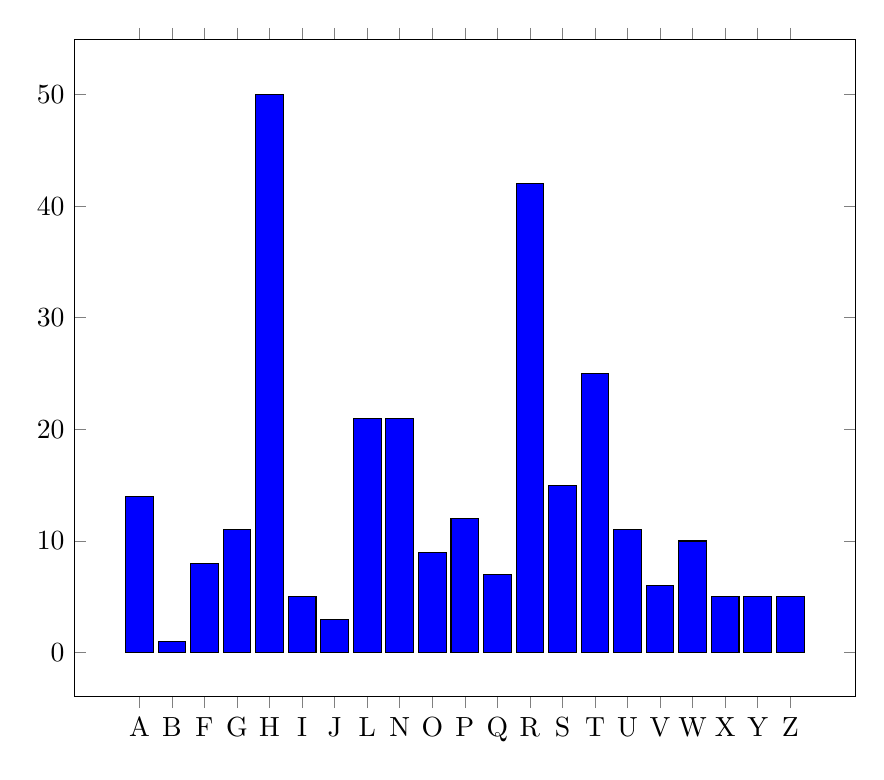
\begin{tikzpicture}
\begin{axis}[
symbolic x coords={
A, B, F, G, H, I, J, L, N, O, P, Q, R, S, T, U, V, W, X, Y, Z
}, xtick=data, ybar=5pt, width=11.5cm
]
\addplot[ybar, fill=blue] coordinates {
(A, 14)
(B, 1)
(F, 8)
(G, 11)
(H, 50)
(I, 5)
(J, 3)
(L, 21)
(N, 21)
(O, 9)
(P, 12)
(Q, 7)
(R, 42)
(S, 15)
(T, 25)
(U, 11)
(V, 6)
(W, 10)
(X, 5)
(Y, 5)
(Z, 5)
};
\end{axis}
\end{tikzpicture}
\caption{Das Säulendiagramm der absoluten Häufigkeiten der Buchstaben aus dem Kryptotext. Kryptotextbuchstaben, die nicht dargestellt sind, haben eine absolute Häufigkeit von \num{0}.}
\label{figure-bsp-historgram}
\end{figure}

Wir können nun vermuten, dass der Kryptotextbuchstabe H im Klartext dem Buchstaben E entspricht. Dies ist deshalb sehr wahrscheinlich, da die absolute Häufigkeit von H in \autoref{figure-bsp-historgram} klar hervorsticht. Wir können jetzt mit dem zweithäufigsten Buchstaben weiterfahren. Dies ist das R. Vermutlich wird dies dem N entsprechen. Weiter können wir noch vermuten, dass das T dem I entspricht. Wir können unsere Vermutungen nun im Kryptotext einsetzen und versuchen erste Wörter zu erraten.

\vfill

\resetlinenumber[1]
\begin{linenumbers}
\small
\_ \_ E I~~~~\_ I N \_ E~~~~\_ E N~~~~E \_ \_ E N \_ \_ E N I \_ E N~~~~\_ \_ \_ \_~~~~I \_~~~~\_ I \_ \_ \_ ,\\
\_ I E \_ E N~~~~\_ E N~~~~\_ \_ E \_ \_ E N \_ E \_ \_ \_ \_ \_ E \_ N~~~~I N~~~~I \_ \_ E N~~~~\_ \_ \_ \_ E N~~~~\_ \_ \_~~~~\_ \_ E I N ,\\
\_ E N~~~~\_ \_ E \_ \_ \_ I \_ \_ E N , E \_ I \_~~~~\_ E \_~~~~\_ \_ \_ E~~~~\_ E \_ \_ \_ \_ \_ E N , N E \_ N ,\\
E I N E \_~~~~\_ E \_~~~~\_ \_ N \_ \_ E N~~~~\_ E \_ \_ N~~~~\_ \_ \_~~~~\_ \_ N \_ \_ E \_~~~~\_ \_ \_ \_ N \\
I \_~~~~\_ \_ N \_ E~~~~\_ \_ \_ \_ \_ \_ , \_ \_~~~~\_ I E~~~~\_ \_ \_ \_ \_ \_ E N~~~~\_ \_ \_ \_ N .\\
E I N~~~~\_ I N \_ , \_ I E~~~~\_ \_~~~~\_ N E \_ \_ \_ E N , \_ I E~~~~\_ \_ \_ E~~~~\_ \_~~~~\_ I N \_ E N ,\\
I N \_~~~~\_ \_ N \_ E \_~~~~\_ \_~~~~\_ \_ E I \_ E N~~~~\_ N \_~~~~E \_ I \_~~~~\_ \_~~~~\_ I N \_ E N \\
I \_~~~~\_ \_ N \_ E~~~~\_ \_ \_ \_ \_ \_ , \_ \_~~~~\_ I E~~~~\_ \_ \_ \_ \_ \_ E N~~~~\_ \_ \_ \_ N .
\end{linenumbers}

\vfill

Die Kryptotextbuchstaben L und N lassen sich in der absoluten Häufigkeit nicht unterscheiden. Wir versuchen nun Bigramme und Trigramme zu zählen. \autoref{figure-bigramme-trigramme-krypto} zeigt die häufigsten Bigramme und Trigramme des Kryptotextes.

\begin{figure}[htb]
\centering
\begin{minipage}{0.45\textwidth}
\centering
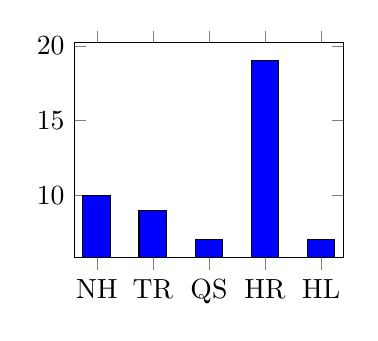
\begin{tikzpicture}
\begin{axis}[
symbolic x coords={
NH, TR, QS, HR, HL
}, xtick=data, ybar=20pt, width=5cm
]
\addplot[ybar, fill=blue] coordinates {
(NH, 10)
(TR, 9)
(QS, 7)
(HR, 19)
(HL, 7)
};
\end{axis}
\end{tikzpicture}
\end{minipage}
\hfill
\begin{minipage}{0.45\textwidth}	
\centering
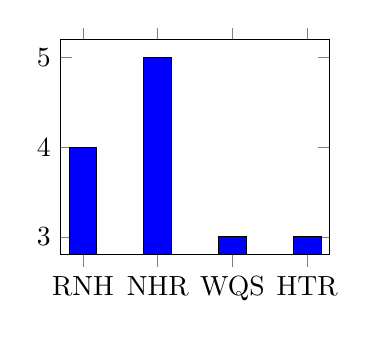
\begin{tikzpicture}
\begin{axis}[
symbolic x coords={
RNH, NHR, WQS, HTR
}, xtick=data, ybar=20pt, width=5cm
]
\addplot[ybar, fill=blue] coordinates {
(RNH, 4)
(NHR, 5)
(WQS, 3)
(HTR, 3)
};
\end{axis}
\end{tikzpicture}
\end{minipage}
\caption{Anzahl der häufigsten Bigramme und Trigramme.}
\label{figure-bigramme-trigramme-krypto}
\end{figure}

Die häufigsten Bigramme in der deutschen Sprache sind ER, EN, CH, TE, ND, EI und DE. Die häufigsten Trigramme sind EIN, ICH, SCH, UND, DIE und NDE. Wir können nun die bereits bestehenden Informationen nutzen, um Bigramme und Trigramme zu erraten. \autoref{table-bigramme-trigramme-krypto} zeigt den aktuellen Stand.

\begin{table}[htb]
\centering
\begin{tblr}{
    colspec = {|l|l|l|l|l|l|l|l|l|l|}
}
\hline
Klartextbuchstaben   & \_ E & IN & \_ \_ & EN & E \_ & N \_ E & \_ EN & \_ \_ \_ & EIN \\ \hline
Kryptotextbuchstaben & NH   & TR & QS    & HR & HL  & RNH  & NHR  & WQS    & HTR \\ \hline
\end{tblr}
\caption{Bigramme und Trigramme kombiniert mit den bestehenden Informationen.}
\label{table-bigramme-trigramme-krypto}
\end{table}

Zwei Bigramme und ein Trigramm wurden bereits mit hoher Wahrscheinlichkeit korrekt erraten. Die Trigramme RNH und NHR teilen sich den noch nicht erratenen Buchstaben N. Ein häufiges Trigramm, welches mit N beginnt und auf E endet, ist NDE. Dies würde auch mit dem Bigramm NH übereinstimmen, da DE ein ebenfalls häufiges Bigramm ist. Ausserdem wäre NHR dann die Verschlüsselung von DEN, was auch plausibel scheint. Wir ersetzen somit N mit einem D. Weiter ist HL noch ein häufiges Bigramm im Kryptotext. Wir vermuten bereits, dass H zu einem E entschlüsselt wird. Somit benötigen wir ein häufiges Bigramm mit dem Anfangsbuchstaben E. Da EN bereits durch HR abgedeckt ist, können wir vermuten, dass HL dem Bigramm ER entspricht. Somit können wir mit hoher Wahrscheinlichkeit davon ausgehen, dass das N zu einem R entschlüsselt werden kann. Wir erhalten mit diesen neuen Informationen folgenden verbesserten Lückentext:

\vfill

\resetlinenumber[1]
\begin{linenumbers}
\small
D R E I~~~~R I N \_ E~~~~D E N~~~~E \_ \_ E N \_ \_ E N I \_ E N~~~~\_ \_ \_ \_~~~~I \_~~~~\_ I \_ \_ \_ ,\\
\_ I E \_ E N~~~~D E N~~~~\_ \_ E R \_ E N \_ E R R \_ \_ \_ E R N~~~~I N~~~~I \_ R E N~~~~\_ \_ \_ \_ E N~~~~\_ \_ \_~~~~\_ \_ E I N ,\\
D E N~~~~\_ \_ E R \_ \_ I \_ \_ E N , E \_ I \_~~~~D E \_~~~~\_ \_ D E~~~~\_ E R \_ \_ \_ \_ E N , N E \_ N ,\\
E I N E R~~~~D E \_~~~~D\_ N \_ \_ E N~~~~\_ E R R N~~~~\_ \_ \_~~~~D \_ N \_ \_ E \_~~~~\_ \_ R \_ N \\
I \_~~~~\_ \_ N D E~~~~\_ \_ R D \_ R , \_ \_~~~~D I E~~~~\_ \_ \_ \_ \_ \_ E N~~~~D R \_ \_ N .\\
E I N~~~~R I N \_ , \_ I E~~~~\_ \_~~~~\_ N E \_ \_ \_ E N , \_ I E~~~~\_ \_ \_ E~~~~\_ \_~~~~\_ I N D E N ,\\
I N \_~~~~D \_ N \_ E \_~~~~\_ \_~~~~\_ R E I \_ E N~~~~\_ N D~~~~E \_ I \_~~~~\_ \_~~~~\_ I N D E N \\
I \_~~~~\_ \_ N D E~~~~\_ \_ R D \_ R , \_ \_~~~~D I E~~~~\_ \_ \_ \_ \_ \_ E N~~~~D R \_ \_ N .
\end{linenumbers}

\vfill

 Wir halten den bisherigen Stand in \autoref{table-caesar-plus-bsp-2} fest.
 
\begin{table}[htb]
\centering
\begin{tblr}{
    colspec = {|c|c|c|c|c|c|c|c|c|c|c|c|c|c|c|c|c|c|c|c|c|c|c|c|c|c|c|}
}
\hline
Klartextbuchstabe & A & B & C & D & E & F & G & H & I & J & K & L & M \\ \hline
Kryptotextbuchstabe &  &  & N & H &  &  &  & T &  &  &  &  &   \\ \hline[2pt]
Klartextbuchstabe & N & O & P & Q & R & S & T & U & V & W & X & Y & Z \\ \hline
Kryptotextbuchstabe & R &  &  &  & L &  &  &  &  &  &  &  &   \\ \hline
\end{tblr}
\caption{Fünf Buchstaben wurden mit hoher Wahrscheinlichkeit bereits geknackt.}
\label{table-caesar-plus-bsp-2}
\end{table}
 
Wir könnten nun weitere Buchstaben, Bigramme und Trigramme untersuchen und so weitere Buchstaben erraten. So könnten wir versuchen, die beiden häufigen Buchstaben S und A als Nächstes zu ermitteln. Wir stoppen das Beispiel an dieser Stelle.
\end{example}

\begin{important}
Das Kryptosystem \texttt{CAESAR-PLUS} ist \textbf{nicht} sicher. Ein Angreifer (Eve) kann mit der Häufigkeitsanalyse den Klartext oder einen Teil davon in vernünftiger Zeit ermitteln.
\end{important}

\subsubsection{Platz für die restliche Kryptoanalyse}

\resetlinenumber[1]
\begin{linenumbers}
\small
D R E I~~~~R I N \_ E~~~~D E N~~~~E \_ \_ E N \_ \_ E N I \_ E N~~~~\_ \_ \_ \_~~~~I \_~~~~\_ I \_ \_ \_ ,\\
\_ I E \_ E N~~~~D E N~~~~\_ \_ E R \_ E N \_ E R R \_ \_ \_ E R N~~~~I N~~~~I \_ R E N~~~~\_ \_ \_ \_ E N~~~~\_ \_ \_~~~~\_ \_ E I N ,\\
D E N~~~~\_ \_ E R \_ \_ I \_ \_ E N , E \_ I \_~~~~D E \_~~~~\_ \_ D E~~~~\_ E R \_ \_ \_ \_ E N , N E \_ N ,\\
E I N E R~~~~D E \_~~~~D\_ N \_ \_ E N~~~~\_ E R R N~~~~\_ \_ \_~~~~D \_ N \_ \_ E \_~~~~\_ \_ R \_ N \\
I \_~~~~\_ \_ N D E~~~~\_ \_ R D \_ R , \_ \_~~~~D I E~~~~\_ \_ \_ \_ \_ \_ E N~~~~D R \_ \_ N .\\
E I N~~~~R I N \_ , \_ I E~~~~\_ \_~~~~\_ N E \_ \_ \_ E N , \_ I E~~~~\_ \_ \_ E~~~~\_ \_~~~~\_ I N D E N ,\\
I N \_~~~~D \_ N \_ E \_~~~~\_ \_~~~~\_ R E I \_ E N~~~~\_ N D~~~~E \_ I \_~~~~\_ \_~~~~\_ I N D E N \\
I \_~~~~\_ \_ N D E~~~~\_ \_ R D \_ R , \_ \_~~~~D I E~~~~\_ \_ \_ \_ \_ \_ E N~~~~D R \_ \_ N .
\end{linenumbers}

\fillwithgrid{\stretch{1}}

\newpage

\subsection{Challenge}

Folgender Kryptotext wurde mit \texttt{CAESAR-PLUS} verschlüsselt. Entschlüsseln Sie den Kryptotext. Tragen Sie einen entschlüsselten Kryptotextbuchstaben in die Tabelle ein. Fassen Sie kurz Ihre Kryptoanalyse zusammen. Hinweise:

\begin{itemize}
	\item Es ist ein Text in deutscher Sprache. Es gilt: ä, ü und ö wurden durch ae, ue und oe ersetzt.
	\item Kommas wurden vor der Verschlüsselung entfernt.
\end{itemize}

\begin{table}[htb]
\centering
\begin{tblr}{
    colspec = {|c|c|c|c|c|c|c|c|c|c|c|c|c|c|c|c|c|c|c|c|c|c|c|c|c|c|c|}
}
\hline
Klartextbuchstabe & A & B & C & D & E & F & G & H & I & J & K & L & M \\ \hline
Kryptotextbuchstabe &  &  &  &  &  &  &  &  &  &  &  &  &   \\ \hline[2pt]
Klartextbuchstabe & N & O & P & Q & R & S & T & U & V & W & X & Y & Z \\ \hline
Kryptotextbuchstabe &  &  &  &  &  & &  &  &  &  &  &  &   \\ \hline
\end{tblr}
\end{table} 

\begin{spacing}{3.25}
\resetlinenumber[1]
\begin{linenumbers}
\ttfamily
UE GOZ UER ZGERMTC NU MNVGRBTEXTV OGUUTE SNTE XLETO RBPMD ZLELGA VLOD GOZ VLE OPEULM DG RTNO RTKE RBPMD RPVLE. ONTULOZ XLTET LGA ZNT NZTT VTWPUUTO RNT WPTOOBTO RNJK NO TNOT UTEWXGTEZNVT GOZ VTKTNUONRSPMMT VTRJKNJKBT STERBENJWTO ZTOO UNB RPMJKTU GORNOO XPMMBTO RNT ONJKBR DG BGO KLFTO. UE ZGERMTC XLE ZNETWBPE TNOTE ANEUL OLUTOR VEGOONOVR ZNT FPKEULRJKNOTO KTERBTMMBT. TE XLE VEPRR GOZ FGMMNV GOZ KLBBT ALRB WTNOTO KLMR ZLAGTE LFTE TNOTO RTKE VEPRRTO RJKOGEEFLEB. UER ZGERMTC XLE ZGTOO GOZ FMPOZ GOZ FTRLRR ZPYYTMB RP SNTM KLMR XNT OPBXTOZNV VTXTRTO XLTET XLR LMMTEZNOVR RTKE OGTBDMNJK XLE ZTOO RP WPOOBT RNT ZTO KLMR GTFTE ZTO VLEBTODLGO ETJWTO GOZ DG ZTO OLJKFLEO KNOGTFTE RYLTKTO. ZNT ZGERMTCR KLBBTO TNOTO WMTNOTO RPKO OLUTOR ZGZMTC GOZ NO NKETO LGVTO VLF TR ONEVTOZXP TNOTO YELTJKBNVTETO HGOVTO.
\end{linenumbers}
\end{spacing}

\newpage

\subsubsection{Lösung}

\begin{spacing}{3.25}
\resetlinenumber[1]
\begin{linenumbers}
\ttfamily
MR UND MRS DURSLEY IM LIGUSTERWEG NUMMER VIER WAREN STOLZ DARAUF GANZ UND GAR NORMAL ZU SEIN SEHR STOLZ SOGAR. NIEMAND WAERE AUF DIE IDEE GEKOMMEN SIE KOENNTEN SICH IN EINE MERKWUERDIGE UND GEHEIMNISVOLLE GESCHICHTE VERSTRICKEN DENN MIT SOLCHEM UNSINN WOLLTEN SIE NICHTS ZU TUN HABEN. MR DURSLEY WAR DIREKTOR EINER FIRMA NAMENS GRUNNINGS DIE BOHRMASCHINEN HERSTELLTE. ER WAR GROSS UND BULLIG UND HATTE FAST KEINEN HALS DAFUER ABER EINEN SEHR GROSSEN SCHNURRBART. MRS DURSLEY WAR DUENN UND BLOND UND BESASS DOPPELT SO VIEL HALS WIE NOTWENDIG GEWESEN WAERE WAS ALLERDINGS SEHR NUETZLICH WAR DENN SO KONNTE SIE DEN HALS UEBER DEN GARTENZAUN RECKEN UND ZU DEN NACHBARN HINUEBER SPAEHEN. DIE DURSLEYS HATTEN EINEN KLEINEN SOHN NAMENS DUDLEY UND IN IHREN AUGEN GAB ES NIRGENDWO EINEN PRAECHTIGEREN JUNGEN.
\end{linenumbers}
\end{spacing}

% ABCDEFGHIJKLMNOPQRSTUVWXYZ
% LFJZTAVKNHWMUOPYIERBGSXQCD

\begin{table}[htb]
\centering
\begin{tblr}{
    colspec = {|c|c|c|c|c|c|c|c|c|c|c|c|c|c|c|c|c|c|c|c|c|c|c|c|c|c|c|}
}
\hline
Klartextbuchstabe & A & B & C & D & E & F & G & H & I & J & K & L & M \\ \hline
Kryptotextbuchstabe & L & F & J & Z & T & A & V & K & N & H & W & M & U  \\ \hline[2pt]
Klartextbuchstabe & N & O & P & Q & R & S & T & U & V & W & X & Y & Z \\ \hline
Kryptotextbuchstabe & O & P & Y & I & E & R & B & G & S & X & Q & C & D  \\ \hline
\end{tblr}
\end{table}

\newpage

\subsection{Aufgaben}

\begin{enumerate}
\item Verschlüsseln Sie den Klartext SCHULFACHINFORMATIK mit dem Kryptosystem \\ \texttt{CAESAR-PLUS} und dem Schlüssel aus folgender Tabelle.

\begin{table}[htb]
\centering
\begin{tblr}{
    colspec = {|c|c|c|c|c|c|c|c|c|c|c|c|c|c|c|c|c|c|c|c|c|c|c|c|c|c|c|}
}
\hline
Klartextbuchstabe 	& A & B & C & D & E & F & G & H & I & J & K & L & M \\ \hline
Kryptotextbuchstabe & P & Z & Q & N & H & J & V & T & A & E & C & O & L  \\ \hline[2pt]
Klartextbuchstabe 	& N & O & P & Q & R & S & T & U & V & W & X & Y & Z \\ \hline
Kryptotextbuchstabe & G & X & B & R & U & I & F & M & W & D & Y & S & K  \\ \hline
\end{tblr}
\end{table}

\fillwithlines{0.25in}

\item Verschlüsseln Sie Ihren Vornamen mit \texttt{CAESAR-PLUS}. Wählen Sie einen eigenen Schlüssel und stellen Sie diesen als Tabelle dar.

\begin{table}[htb]
\centering
\begin{tblr}{
    colspec = {|c|c|c|c|c|c|c|c|c|c|c|c|c|c|c|c|c|c|c|c|c|c|c|c|c|c|c|}
}
\hline
Klartextbuchstabe & A & B & C & D & E & F & G & H & I & J & K & L & M \\ \hline
Kryptotextbuchstabe &  &  &  &  &  &  &  &  &  &  &  &  &   \\ \hline[2pt]
Klartextbuchstabe & N & O & P & Q & R & S & T & U & V & W & X & Y & Z \\ \hline
Kryptotextbuchstabe &  &  &  &  &  & &  &  &  &  &  &  &   \\ \hline
\end{tblr}
\end{table}

\fillwithlines{0.25in}

\item Der Klartext ANDIESTIFTEFERTIGLOS wurde mit dem Kryptosystem \texttt{CAESAR-PLUS} zum Kryptotext ERBLZDILXIZXZJILGTVD verschlüsselt. Was können Sie über den verwendeten Schlüssel erfahren?

\fillwithlines{0.25in}

\begin{table}[htb]
\centering
\begin{tblr}{
    colspec = {|c|c|c|c|c|c|c|c|c|c|c|c|c|c|c|c|c|c|c|c|c|c|c|c|c|c|c|}
}
\hline
Klartextbuchstabe & A & B & C & D & E & F & G & H & I & J & K & L & M \\ \hline
Kryptotextbuchstabe &  &  &  &  &  &  &  &  &  &  &  &  &   \\ \hline[2pt]
Klartextbuchstabe & N & O & P & Q & R & S & T & U & V & W & X & Y & Z \\ \hline
Kryptotextbuchstabe &  &  &  &  &  & &  &  &  &  &  &  &   \\ \hline
\end{tblr}
\end{table}

\item Beenden Sie die Häufigkeitsanalyse aus \autoref{example-hdr} und bestimmen Sie den Klartext. Sie finden am Ende des Beispiels Platz für Ihre Analyse.

\item Entwickeln Sie für das Klartextalphabet der Dezimalziffern (0, 1, 2, 3, 4, 5, 6, 7, 8, 9) ein monoalphabetisches Kryptosystem mit vielen Schlüsseln ($|\mathscr{S}| \geq 10^6$). Sie dürfen das Kryptotextalphabet selbst wählen. Erklären Sie, wie verschlüsselt und entschlüsselt wird. Bestimmen Sie auch die exakte Grösse der Schlüsselmenge.

\fillwithgrid{\stretch{1}}

\newpage

\item Der folgende Klartext wurde mit dem Kryptosystem \texttt{CAESAR-PLUS} aus einem deutschen Klartext erzeugt. Machen Sie auf einem separaten Notizpapier eine Häufigkeitsanalyse und bestimmen Sie so den Klartext.

\begin{spacing}{3.25}
\resetlinenumber[1]
\begin{linenumbers}
\ttfamily
HOQ HQKSD, DOCOPTSPXXO KERJEHOLZOS, PXN PT VOXOS HOX\\
TOSXLCOS NPOR OPSDOVEQJOIN; XLCMS HPO OPSRKLCXNO SOEDPOQ\\
WOQECN UK KER HOQ KEXXPLCN, OPS VPXXOS JE NOPIOS,\\
HKX KSHOQO ESX YMQOSNCKINOS. OPSPDO XPSH DIEOLZIPLC DOSED,\\
OPSOS WOQER JE RPSHOS, HOQ PS HOQ IMOXESD YMS QKONXOIS\\
WOXNOCN. KWOQ HPO TOPXNOS YMS ESX TEOXXOS HPOXOS HQKSD TPN\\
HOQ IMOXESD ZEOSXNIPLC JE ESXOQOQ ESNOQCKINESD\\
KEXDOHKLCNOQ QKONXOIKERDKWOS XNPIIOS. HONOZNPYDOXLCPLCNOS\\
ESH ZQOEJVMQNQKONXOI VOQHOS YPOIOS SENJOS;\\
OPSPDO VOSPDO TMODOS XPLC HOQ OSNXLCIEOXXOIESD\\
YMS DOCOPTXLCQPRNOS CPSDOWOS.
\end{linenumbers}
\end{spacing}

\newpage

\item Der folgende Klartext wurde mit dem Kryptosystem \texttt{CAESAR-PLUS} aus einem deutschen Klartext erzeugt. Machen Sie auf einem separaten Notizpapier eine Häufigkeitsanalyse und bestimmen Sie so den Klartext.

\begin{spacing}{3.25}
\resetlinenumber[1]
\begin{linenumbers}
\ttfamily
GP ETM GLRXTN QIM NTRJGM BGLA LR GLRGM EGLA, EGLA GRAZGMRAGR JTNTSLP. PATM ETMP. GULPIFG LQ. GLRG RGWG YIZZRWRJ\\
GP YGMMPKYA VWGMJGMHMLGJ. FLG MGVGNNGR, FGMGR MTWXPKYLZZG QIR GLRGX JGYGLXGR PAWGABUWRHA TWP TRJMGLZGR, YTVGR LYMGR GMPAGR PLGJ JGJGR FTP VIGPG JTNTHALPKYG LXUGMLWX GMMWRJGR.\\
ETGYMGRF FGM PKYNTKYA LPA GP PULIRGR FGM MGVGNNGR JGNWRJGR, JGYGLXUNTGRG WGVGM FLG TVPINWAG ETZZG FGP LXUGMLWXP LR LYMGR VGPLAB BW VMLRJGR, FGR AIFGPPAGMR, GLRG VGETZZRGAG MTWXPATALIR, FGMGR ZGWGMHMTZA TWPMGLKYA, WX GLRGR JTRBGR UNTRGAGR BW QGMRLKYAGR.\\
QGMZINJA QIR FGR ZLRPAGMGR TJGRAGR FGP LXUGMLWXP, GLNA UMLRBGPPLR NGLT TR VIMF LYMGP PAGMRGRPKYLZZP LR LYMG YGLXTA, TNP YWGAGMLR FGM GMVGWAGAGR UNTGRG, FLG LYM QINH MGAAGR WRF FGM JTNTSLP FLG ZMGLYGLA ELGFGMJGVGR HIGRRAGR.
\end{linenumbers}
\end{spacing}

%ES WAR EINMAL VOR LANGER ZEIT IN EINER WEIT, WEIT ENTFERNTEN GALAXIS. STAR WARS. EPISODE IV. EINE NEUE HOFFNUNG.
%ES HERRSCHT BUERGERKRIEG. DIE REBELLEN, DEREN RAUMSCHIFFE VON EINEM GEHEIMEN STUETZPUNKT AUS ANGREIFEN, HABEN IHREN ERSTEN SIEG GEGEN DAS BOESE GALAKTISCHE IMPERIUM ERRUNGEN.
%WAEHREND DER SCHLACHT IST ES SPIONEN DER REBELLEN GELUNGEN, GEHEIMPLAENE UEBER DIE ABSOLUTE WAFFE DES IMPERIUMS IN IHREN BESITZ ZU BRINGEN, DEN TODESSTERN, EINE BEWAFFNETE RAUMSTATION, DEREN FEUERKRAFT AUSREICHT, UM EINEN GANZEN PLANETEN ZU VERNICHTEN.
%VERFOLGT VON DEN FINSTEREN AGENTEN DES IMPERIUMS, EILT PRINZESSIN LEIA AN BORD IHRES STERNENSCHIFFS IN IHRE HEIMAT, ALS HUETERIN DER ERBEUTETEN PLAENE, DIE IHR VOLK RETTEN UND DER GALAXIS DIE FREIHEIT WIEDERGEBEN KOENNTEN.
%
%abcdefghijklmnopqrstuvwxyz
%tvkfgzjylohnxriucmpawqesdb

\end{enumerate}
